%%%%%%%%%%%%%%%%%%%%%%%%%%%%%%%%%%%%%%%%%%%%%%%%%%%
%%%%%   STUDY DESIGN & EXPLORATORY ANALYSIS   %%%%%
%%%%%%%%%%%%%%%%%%%%%%%%%%%%%%%%%%%%%%%%%%%%%%%%%%%
\chapter{Study design and description}
\label{ch:2.0}

Including the island of Zanzibar, Tanzania has almost 42 million inhabitants.
Tanzania is an East African country with moderate malaria endemicity \cite{sicuri2013economic}.
Throughout the past decades, Tanzania has made important progresses towards malaria control \cite{worldbank2017}.
%\textbf{cite: Combined Project Information Documents / Integrated Safeguards Datasheet (PID/ISDS)}.
From early 2000 until 2010, initiatives provided campaigns and interventions such as distribution of bed nets for mosquito control and improvement of diagnostics and treatment that allowed the country to gradually reduce its proportion of communities living in areas of intense transmission \cite{world2013epidemiological}.
Recent data suggests almost 60\% of the population currently lives in low transmission settings \cite{world2013epidemiological}.
The data used throughout this project were collected between 2001 and 2002 as part of a program investigating the burden of malaria and its transmission intensity across 24 villages in Tanzania \cite{drakeley2005altitude}.

%%%%%%%%%%%%%%%%%%%%
% TANZANIA DATASET %
%%%%%%%%%%%%%%%%%%%%
\section{Tanzania data set}

%%%%%%%%%%%%%%%%%%%%
\subsection{Study sites on Northeast Tanzania}

Within the Northeast Tanzania, the study encompassed the Kilimanjaro region, an inland area with the highest mountain in Africa, and the Tanga region, with the Usambara mountains and coastal plains near the Indian Ocean.
% \cite{world2013epidemiological}.
Six transects were delimited: Rombo, North, and South Pare in the Kilimanjaro region, and West Usambara 1, 2, and 3 in the Tanga region.
Each transect containing four villages located at different altitudes. One at high altitude ($>$1200m), two at intermediate altitude (600m$-$1200m), and one the closest to a low altitude ($<$600m) (Figure \ref{fig:tanzania.map}).
All transects comprised nearby areas with varying transmission intensity, representing increasing prevalence from high to low altitude.
%based on the premise that the effect of increasing altitude follows a reduction in \textit{Anopheles} vectors density and consequent fall in malaria transmission.
Each village was measured for its mean altitude, daily mean temperature, and rainfall estimates, derived from meteorological stations across both regions.
\vfill


%%%%%%%%%%%%%%%%%%%%
\subsection{Cross-sectional survey}

Two cross-sectional surveys were conducted in each village.
A first one after the short rainy season in November of 2001, and a second during the following year in June, after the long rains.
% The surveys were age-stratified for each village.
%age-stratified malariometric surveys were conducted in each village.
In addition to the local geographical data, for each one of the 24 villages the study objectives were to collect clinical and anthropometric data, as well as blood samples from a total of approximately 250 inhabitants, all structured by age: 80 with ages between 0$-$4 years old, 80 who were between 5$-$14 years old, and 90 who were between 15$-$45 years old.
The corresponding populational sampling proportions were then approximately 30\%, 30\%, and 40\%. 
% \textcolor{red}{Isto eram os objectivos, o que foi planeado (tenho de fazer referência à diferença entre planeamento e execução.}
Attention so that the sexes kept the same ratio across villages was also taken in account, being achieved in the younger age groups, although approximately 70\% of the 15$-$45 years old group surveyed were women.
Within each transect a selection criteria was taken to minimise differences in ethnicity.
This granted a dominant ethnic group between villages in the same transect, reducing the genetic diversity across those geographically closer sites.
Seasonal migration, and access to health care were also points taken into account during the population sampling.
%The study was able to collect several demographical indices (altitude levels, estimated daily temperatures, estimated annual rainfall) for each one of the 24 villages), as well as specific and proportioned age-stratified information for the different populations, including individual values such as age, gender, marital status, height, weight, body temperature, haemoglobin levels, presence/absence of malaria infection and specific antibodies to the malaria antigens.\\

\begin{figure}[!hb]
\center
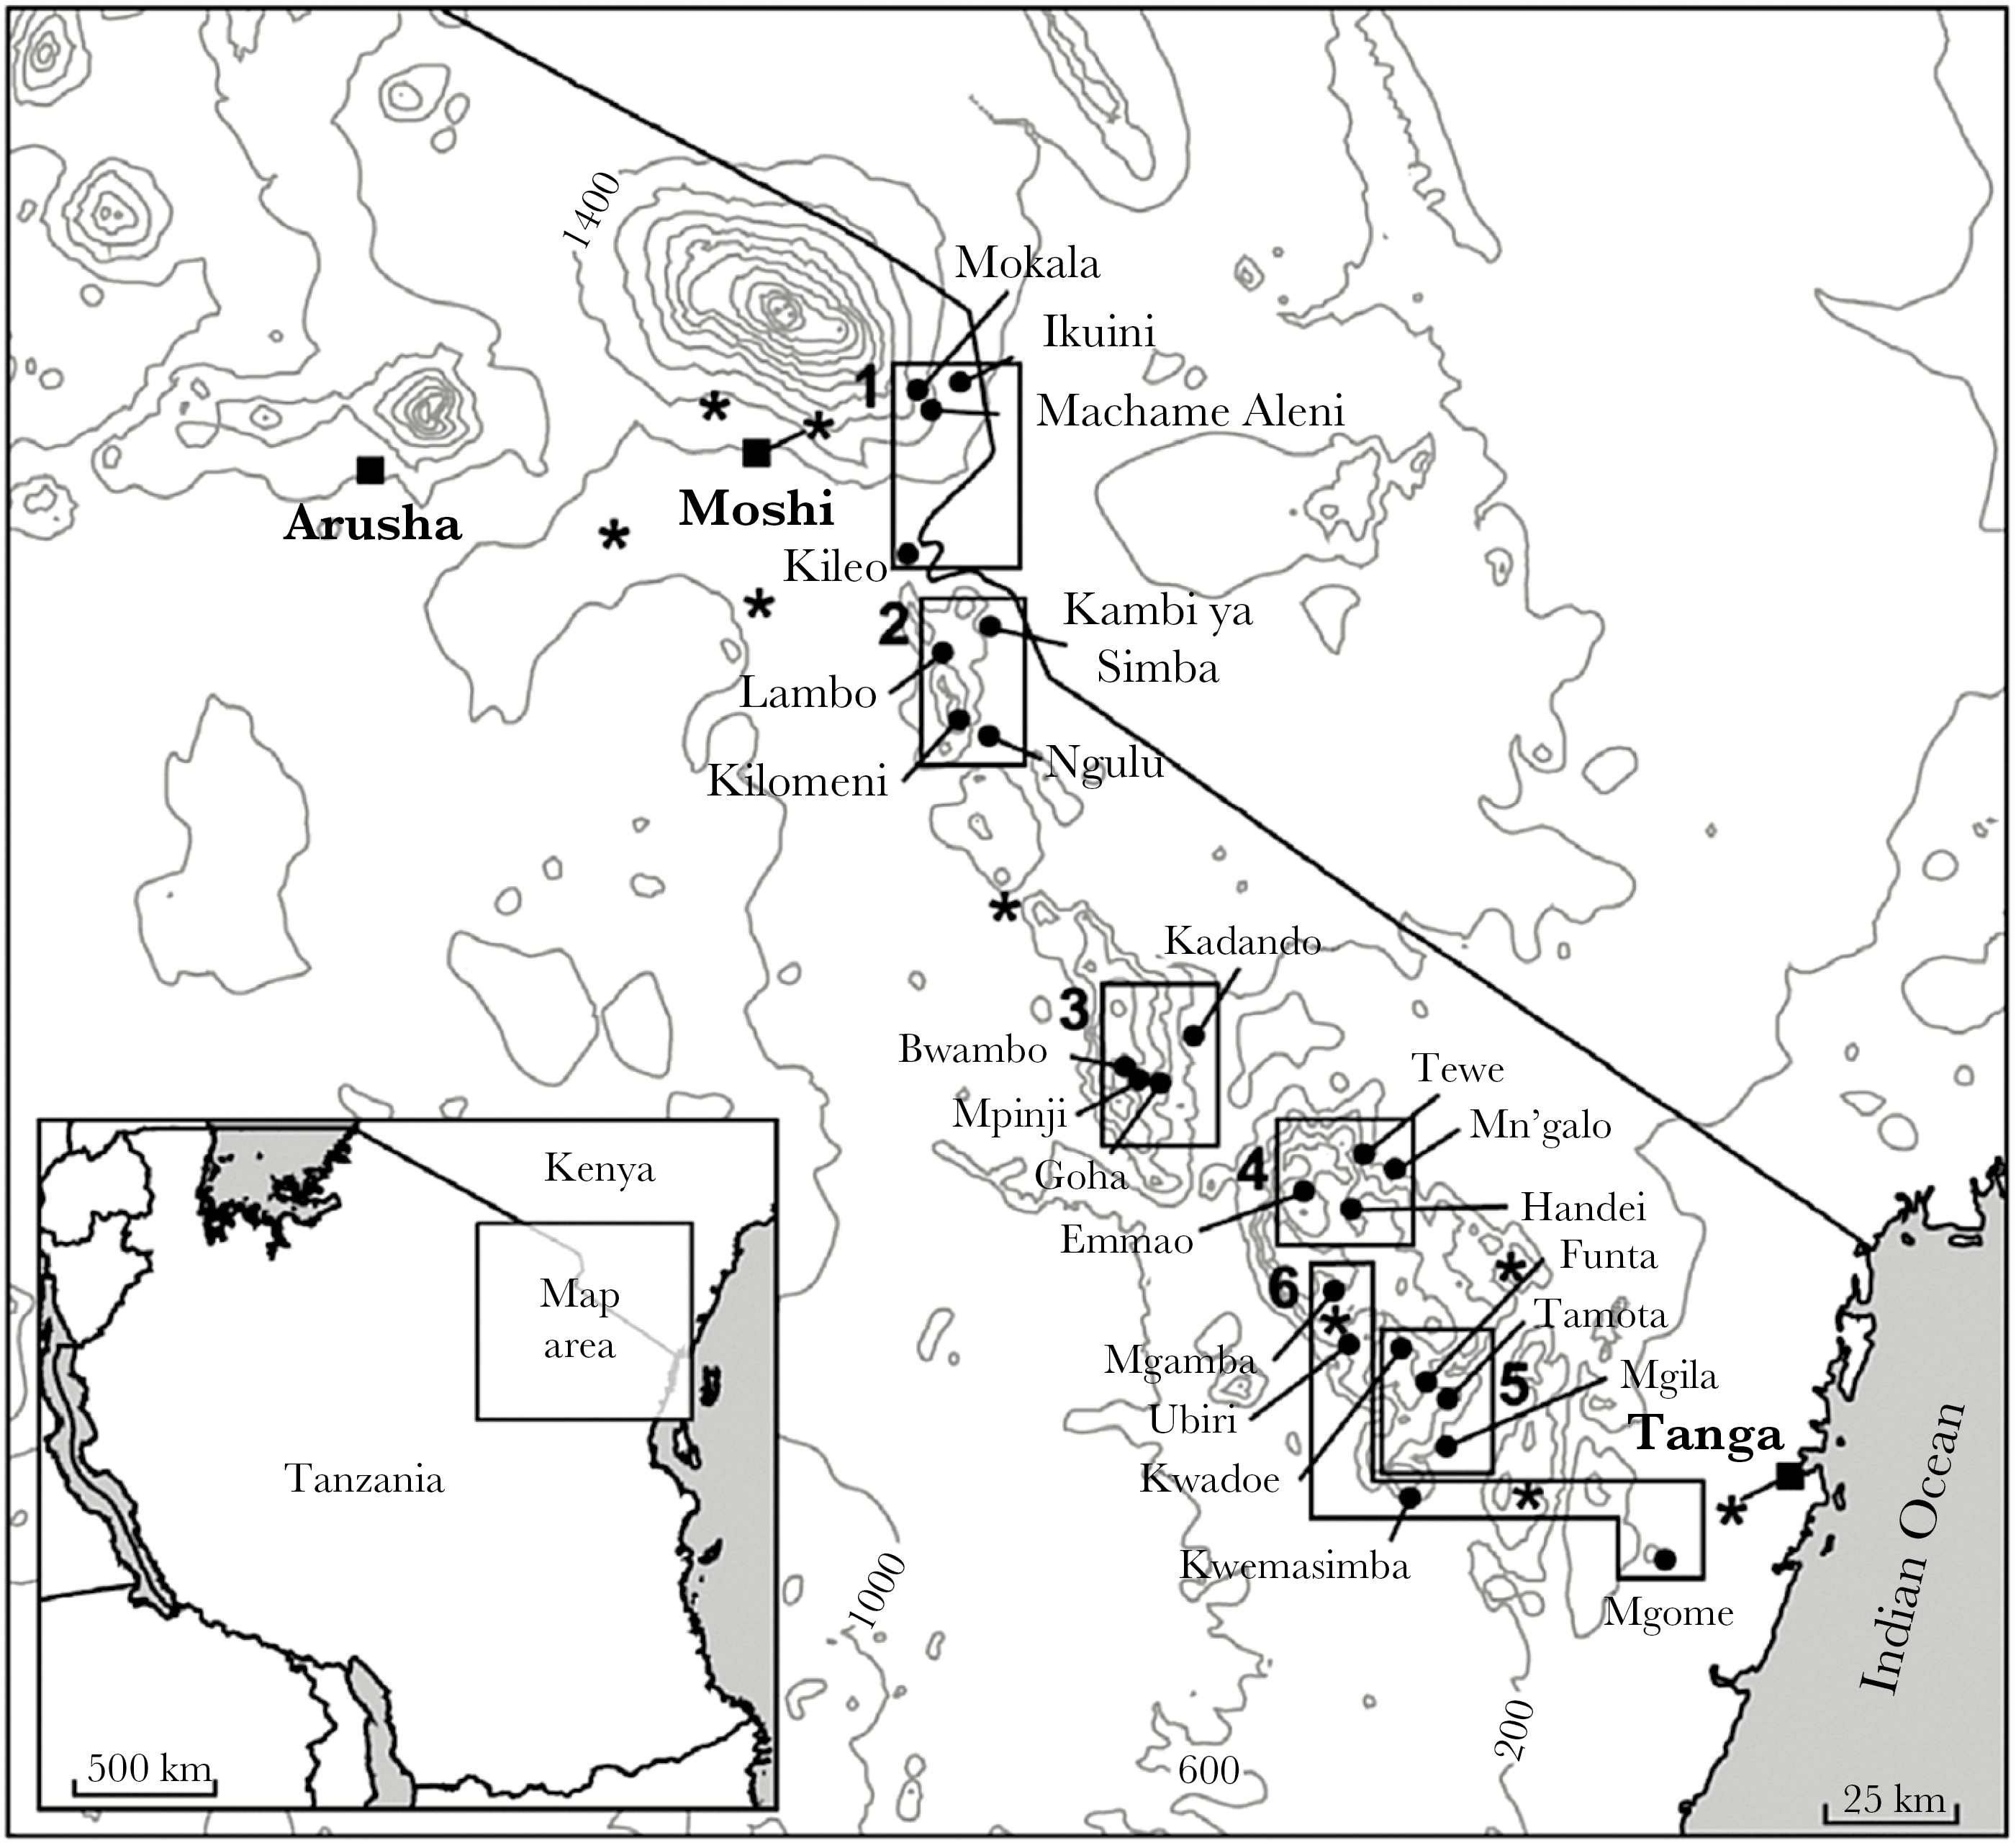
\includegraphics[width=13cm]{images/site_map.jpeg}
\caption[Map of study sites]{Map of study sites (black circles) grouped by respective numbered region transects: Rombo (transect 1), North Pale (transect 2), South Pale (transect 3), West Usambara 1 (transect 4), West Usambara 2 (transect 5), and West Usambara 3 (transect 6).
Locations of the 8 meteorological stations are also shown (asterisks).
Reprinted with permission \cite{sepulveda2017malaria}.}
\label{fig:tanzania.map}
\end{figure}



%%%%%%%%%%%%%%%%%%%%%%%%%
% VARIABLES DESCRIPTION %
%%%%%%%%%%%%%%%%%%%%%%%%%

%\section{Descriptive analysis}
\section{Variables description}

To study transmission intensity amongst Tanzania's different populations, several variables were selected to be analysed in this thesis.
Some variables refer the demographical information collected regarding each site.
For each village, its mean altitude and encompassing transect were registered.
Variables that characterise the selected inhabitants were also used.
Firstly, the infection outcome recorded for each individual.
This variable has value 0 in absence of infection and 1 when presence of malaria parasites is found, indicating the assumed true individual status.
Other binary variables selected were the gender of each individual (as female or male), and the three \textit{P. falciparum} antigens (either present or absent), used here as serological markers to identify exposure to parasite instead of immunological protection.
Since each antigen has different response levels to the presence of \textit{P. falciparum} parasites, the comparison of their serological outcomes under the same study characteristics could help to better understand how transmission intensity varies across the different villages.
Ethnicities were also recorded, with four possible ethnic groups: Wachaga, Wapare, Wasambaa, and Other.
As mentioned in the previous section, the ethnic groups of each village are expected to represent the genetic variability seen in each transect.
In other words, in each transect an ethnic group dominated the others in proportion.
The age in years of every individual was also a recorded variable, as well as the respective age group each one belonged to, with three possible categories, 1$-$4, 5$-$14, and 15$-$45.

Depending on the study objective, more than one of the described variables can be classified as the desired response variable, with others being used as explanatory variables and potential risk factors.
An example of response variable can be the infection or serological status of each individual.
The binary outcomes of these variables can be used to calculate the number of infected or previously exposed individuals within each village, attending other particular variables that may characterise such response.
All ten variables considered for the analyses are listed below.
%\subsubsection{Outcomes of interest}
%To study the transmission intensity amongst Tanzania's population, the response variable used was the number of infected individuals at each age group.
%This variable is dependent on the outcome for \textit{P. falciparum} infection, with possible values 0 in absence of infection and 1 when presence of malaria parasites is found.
%The outcome indicates the assumed true individual status.
%The use of this variable has a direct use when estimating malaria transmission intensity via the more classical epidemiological measures.
%\textbf{falar também das serologias!}
%\subsubsection{Covariates}
%Alongside the infection status a number of potential explanatory variables were recorded for each individual.
%These covariates can be separated in two distinct groups regarding the information they contain: demographical variables and epidemiological variables.
%The demographical variables the all the information collected regarding the sites and its inhabitants.
%Included in this group are the mean altitude of each village, the different transects, the three age groups, the individuals' gender, and their respective ethnicity.
%The epidemiological variables refer the three specific \textit{P. falciparum} antigens screened: PfMSP1, PfMSP2, and PfAMA1.
%Similar to the infection status, the epidemiological variables were registered for all individuals as 0 when it is not detectable, and 1 if it is.
%The explanatory variables used in the analyses are briefly listed listed below.
%\setlist[description]{font=\normalfont\itshape\space, leftmargin=\parindent,labelindent=\parindent}
%
\setlist[description]{labelindent=0pt,style=multiline,leftmargin=1.9cm}
\begin{description}[font=\normalfont\itshape]
\item [Altitude:]  Mean altitude of each village, in meters;
\item [Transect:]  Transect of villages (categorical variable with six possible outcomes, Rombo, North Pare, South Pare, West Usambara 1, West Usambara 2, and West Usambara 3);
\item [Gender:]  Gender of each individual (binary variable with possible outcomes, Female and Male);
\item [EthGp:]  Ethnic group of each individual (categorical variable with four possible outcomes, Wachaga, Wapare, Wasambaa, and Other);
\item [AgeYears:]  Age of each individual, in years;
\item [AgeGp:]  Age group of each individual (categorical variable with three possible outcomes, 1$-$4, 5$-$14, and 15$-$45);
\item [Infection:]  Infection status of each individual (binary variable with possible outcomes, 0 = infection is absent, and 1 = \textit{P. falciparum} malaria detected);
\item [MSP1:]  Serological status regarding the antigen MSP1 (binary variable with possible outcomes, 0 = antigen absent in serum, and 1 = antigen detected);
\item [MSP2:]  Serological status regarding the antigen MSP2 (binary variable with possible outcomes, 0 = antigen absent in serum, and 1 = antigen detected);
\item [AMA1:]  Serological status regarding the antigen AMA1 (binary variable with possible outcomes, 0 = antigen absent in serum, and 1 = antigen detected).
\end{description}

%%%%%%%%%%%%%%%%%%%%%%%%
% EXPLORATORY ANALYSIS %
%%%%%%%%%%%%%%%%%%%%%%%%
\section{Exploratory analysis}

The decision to perform analyses using only the complete cases for the described variables led to the exclusion of three villages from the West Usambara 3 transect (the villages removed were Magamba, Ubiri and Kwemasimba), where serological samples were not collected.
In this transect the remaining village, Mgome, is a coastal village with the lowest recorded mean altitude, at 179 meters.
By comparison, the first transect of the Usambara mountains registers the village located at highest altitude, Emmao, at 1780 meters high.
The resulting total population sample size is 5058 individuals, separated across the 21 villages (Table \ref{tab:demographic}).
Considering each village, the sample sizes ranged from 53 (Ngulu) up to 379 individuals (Handei).
Even with different sample sizes it was possible to verify the attention taken by the study to maintain a similar structure for ages and genders, as these variables presented similar proportions across all sites.
Similar attention was also taken for the different ethnic groups within each one of the six transects.
Each transect had a dominant ethnicity.
Rombo was represented by the Wachaga ethnic group, having only one village (Kileo) with Wapare as the main ethnicity, North and South Pare had mostly individuals from the Wapare ethnic group, both West Usambara 1 and 2 had Wasambaa as the main ethnic group, and the last transect, West Usambara 3, represented a mixture of different ethnicities (Other).
\\

\begin{table}[ht!]
\centering
\caption[Variables recorded for each village]{Descriptive table with the recorded variables for each one of the 21 selected villages within six different transects.
For all villages, values for mean altitude, population sample size, gender proportion, mean age, and proportion of each ethnic group are presented.}
\label{tab:demographic}
\begin{adjustbox}{width=1\linewidth}
\begin{tabular}{llccrcrrrr} 
\toprule
\multicolumn{1}{c}{\multirow{2}{*}{Transect}} & \multicolumn{1}{c}{\multirow{2}{*}{Village}} & \multirow{2}{*}{\begin{tabular}[c]{@{}c@{}} Altitude,\\m\end{tabular}} & \multirow{2}{*}{$n$} & \multirow{2}{*}{\begin{tabular}[c]{@{}c@{}} Female\\proportion, \% ($n$)\end{tabular}} & \multirow{2}{*}{\begin{tabular}[c]{@{}c@{}} Mean age,\\years\end{tabular}} & \multicolumn{4}{c}{Ethnic group, \% ($n$)}  \\ 
\cmidrule{7-10}
                          & \multicolumn{1}{c}{}   &   &   &   &   &   \multicolumn{1}{c}{Wachaga}   &   \multicolumn{1}{c}{Wapare}   &   \multicolumn{1}{c}{Wasambaa}   &   \multicolumn{1}{c}{Other}   \\ 
\midrule
Rombo                     &   Mokala          &   1703   &   291   &   62.20 (181)   &   15.34   &   98.28 (286)&   0.00 (0)    &   0.00 (0)   &   1.72 (5)     \\
                          &   Machame Aleni   &   1422   &   225   &   55.11 (124)   &   15.28   &   100.00 (225)  &   0.00 (0)    &   0.00 (0)   &   0.00 (0)   \\
                          &   Ikuini          &   1160   &   256   &   57.03 (146)   &   14.99   &   98.83 (253)&   0.39 (1)    &   0.39 (1)    &   0.39 (1)     \\
                          &   Kileo           &   723    &   223   &   61.88 (138)   &   14.94   &   3.14 (7)   &   86.55 (193) &   5.38 (12)   &   4.93 (11)    \\
\cmidrule{2-10}
N. Pare                   &   Kilomeni        &   1556   &   101   &   55.45 (56)    &   17.71   &   0.99 (1)   &   96.04 (97)  &   0.99 (1)    &   1.98 (2)     \\
                          &   Lambo           &   1188   &   131   &   64.89 (85)    &   15.43   &   0.00 (0)   &   94.66 (124) &   1.53 (2)    &   3.82 (5)     \\
                          &   Ngulu           &   832    &   53    &   52.83 (28)    &   13.75   &   1.89 (1)   &   96.23 (51)  &   1.89 (1)    &   0.00 (0)   \\
                          &   Kambi ya Simba  &   746    &   93    &   50.54 (47)    &   15.43   &   6.45 (6)   &   81.72 (76)  &   0.00 (0)   &   11.83 (11)   \\
\cmidrule{2-10}
S. Pare                   &   Bwambo          &   1598   &   240   &   54.17 (130)   &   16.61   &   1.25 (3)   &   98.33 (236  &   0.00 (0)   &   0.42 (1)     \\
                          &   Mpinji          &   1445   &   198   &   63.13 (125)   &   14.03   &   0.51 (1)   &   93.94 (186) &   2.02 (4)    &   3.54 (7)     \\
                          &   Goha            &   1163   &   337   &   58.75 (198)   &   14.53   &   0.00 (0)   &   96.44 (325) &   2.97 (10)   &   0.59 (2)     \\
                          &   Kadando         &   528    &   281   &   59.07 (166)   &   16.19   &   1.42 (4)   &   69.40 (195) &   18.51 (52)  &   10.68 (30)   \\
\cmidrule{2-10}
W. Usamb. 1               &   Emmao           &   1780   &   170   &   61.18 (104)   &   16.04   &   0.00 (0)   &   15.29 (26)  &   60.00 (102) &   24.71 (42)   \\
                          &   Handei          &   1368   &   379   &   56.46 (214)   &   14.21   &   0.00 (0)   &   2.11 (8)    &   94.20 (357) &   3.69 (14)    \\
                          &   Tewe            &   999    &   326   &   61.96 (202)   &   15.68   &   0.31 (1)   &   3.07 (10)   &   93.56 (305) &   3.07 (10)    \\
                          &   Mn'galo         &   389    &   363   &   58.95 (214)   &   15.58   &   0.00 (0)   &   1.10 (4)    &   89.53 (325) &   9.37 (34)    \\
\cmidrule{2-10}
W. Usamb. 2               &   Kwadoe          &   1564   &   296   &   62.16 (184)   &   15.14   &   0.68 (2)   &   2.03 (6)    &   94.59 (280) &   2.70 (8)     \\
                          &   Funta           &   1240   &   252   &   66.67 (168)   &   15.90   &   0.40 (1)   &   0.40 (1)    &   96.43 (243) &   2.78 (7)     \\
                          &   Tamota          &   1055   &   330   &   53.94 (178)   &   15.62   &   0.61 (2)   &   1.21 (4)    &   94.55 (312) &   3.64 (12)    \\
                          &   Mgila           &   375    &   288   &   71.88 (207)   &   15.62   &   0.00 (0)   &   9.72 (28)   &   67.36 (194) &   22.92 (66)   \\
\cmidrule{2-10}
W. Usamb. 3               &   Mgome           &   179    &   225   &   54.22 (122)   &   15.46   &   0.44 (1)   &   5.33 (12)   &   9.78 (22)   &   84.44 (190)  \\
\bottomrule
\end{tabular}
\end{adjustbox}
\end{table}

The combination of characteristics from each site may have different impacts in the resulting prevalence of infection, changing the seroprevalence values as consequence (Table \ref{tab:prevalence.categories}).
The overall prevalence of infection was reported as 19.81\%, with seroprevalence values for MSP1, MSP2, and AMA1 being 36.22\%, 40.25\%, and 46.56\%, respectively.
% The confidence intervals for the prevalence and seroprevalence values represent the uncertainty based on the sample size at each category, calculated for a significance level fixed at 0.05.
Analysing the different categories showed that \textit{Gender} did not seem to pose an effect on neither prevalence nor seroprevalence, as both estimates did not change much from female individuals to males.
Prevalence of infection across ethnic groups (variable \textit{EthGp}), showing different registered sample sizes, suggested mixed ethnicities ($\textit{EthGp}_{Other}$) suffered the most from detectable cases, presenting higher seroprevalence levels as well.
% As previously described, this ethnic group represents the last of the West Usambara transects, with only the village of Mgome.

% The change in prevalence across different age groups (\textit{AgeGp}) suggests evidence for the previously referred peak-shift effect.
% A justification might be the gradual increase in seroprevalence from one age group to the following.
Since individuals are born almost immunologically unprotected, with only maternal antibodies inherited from the mother, the first age group ($\textit{AgeGp}_{1-4}$) showed lower seroprevalence values.
Contrarily, the last age group ($AgeGp_{15-45}$) had a reduced prevalence of infection, with over 50\% of this older population showing presence of the various antimalarial antigens.
In this particular scenario, the difference in prevalence and seroprevalence between age groups might be justified by the gradual accumulation of protective antibodies due to exposure over time.
The primary risk group in these African populations is then children younger than 5 years old, who have yet to develop an efficient immune system \cite{snow2002consequences}.
Pregnant woman can also be a vulnerable group to malaria infections, as pregnancy affects the immune system's defences against the disease \cite{carter2002evolutionary,perlmann2002malaria}.
This influence of age on prevalence of infection and seroprevalence can be seen as the previously described peak-shift.
As malaria does not produce long-lasting immunity, in a case of transmission intensity reduction (or eradication), the developed (and accumulated) antibodies for the specific antigens could gradually decay, with the immunologically protected individuals becoming susceptible to high and symptomatic cases of infection, once again.

\begin{table}[H]
\centering
\caption[Prevalence and seroprevalence for each categorical variable]{Prevalence and seroprevalence of each one of the specific \textit{P. falciparum} antigens, estimated for the categorised available variables. Each prevalence and seroprevalence shows the 95\% confidence interval (CI), estimated using the Wald interval.}
\label{tab:prevalence.categories}
\begin{adjustbox}{width=1\linewidth}
\begin{tabular}{llcrrrr} 
\toprule
\multicolumn{1}{c}{\multirow{2}{*}{Variables}} & \multicolumn{1}{c}{\multirow{2}{*}{Categories}} & \multicolumn{1}{c}{\multirow{2}{*}{$n$}} & \multicolumn{1}{c}{\multirow{2}{*}{\begin{tabular}[c]{@{}c@{}}Prevalence, \%\\ (95\% CI) \end{tabular}}} & \multicolumn{3}{c}{Seroprevalence, \% (95\% CI)}                                \\ 
\cmidrule{5-7}
\multicolumn{1}{c}{} & \multicolumn{1}{c}{} & \multicolumn{1}{c}{} & \multicolumn{1}{c}{} & \multicolumn{1}{c}{MSP1} & \multicolumn{1}{c}{MSP2} & \multicolumn{1}{c}{AMA1}  \\ 
\midrule
\textit{AgeGp}                                 & 1$-$4         &   1261   & 19.59 (17.40, 21.78)   & 19.83 (17.63, 22.03)   & 24.27 (21.90, 26.63)   & 30.61 (28.07, 33.15)   \\
                                               & 5$-$14        &   1789   & 25.88 (23.85, 27.91)   & 30.58 (28.44, 32.71)   & 39.18 (36.92, 41.45)   & 45.78 (43.47, 48.09)   \\
                                               & 15$-$45       &   2008   & 14.54 (13.00, 16.08)   & 51.54 (49.36, 53.73)   & 51.25 (49.06, 53.43)   & 57.27 (55.11, 59.43)   \\
\textit{Gender}                                & Female      &   3017   & 18.99 (17.59, 20.39)   & 38.88 (37.14, 40.62)   & 42.46 (40.70, 44.22)   & 47.99 (46.21, 49.78)   \\
                                               & Male        &   2041   & 21.02 (19.25, 22.79)   & 32.29 (30.26, 34.32)   & 36.99 (34.90, 39.09)   & 44.44 (42.28, 46.59)   \\
\textit{EthGp}                                 & Wachaga     &   794    & 6.68 (4.94, 8.41)      & 20.03 (17.24, 22.81)   & 4.28 (2.87, 5.69)      & 7.68 (5.83, 9.54)      \\
                                               & Wapare      &   1583   & 9.85 (8.39, 11.32)     & 34.30 (31.96, 36.64)   & 39.48 (37.07, 41.89)   & 47.38 (44.92, 49.84)   \\
                                               & Wasambaa    &   2223   & 28.39 (26.51, 30.26)   & 38.46 (36.44, 40.48)   & 48.13 (46.06, 50.21)   & 55.29 (53.22, 57.35)   \\
                                               & Other       &   458    & 35.37 (30.99, 39.75)   & 60.04 (55.56, 64.53)   & 67.03 (62.73, 71.34)   & 68.78 (64.53, 73.02)   \\
\textit{Transect}                              & Rombo       &   995    & 6.73 (5.18, 8.29)      & 31.26 (28.38, 34.14)   & 4.82 (3.49, 6.16)      & 10.35 (8.46, 12.24)    \\
                                               & N. Pare     &   378    & 4.76 (2.62, 6.91)      & 28.31 (23.77, 32.85)   & 38.36 (33.46, 43.26)   & 54.23 (49.21, 59.26)   \\
                                               & S. Pare     &   1056   & 11.74 (9.80, 13.68)    & 29.64 (26.89, 32.39)   & 45.17 (42.17, 48.17)   & 49.91 (46.89, 52.92)   \\
                                               & W. Usamb. 1 &   1238   & 32.31 (29.71, 34.92)   & 29.08 (26.55, 31.61)   & 40.39 (37.65, 43.12)   & 65.75 (63.11, 68.39)   \\
                                               & W. Usamb. 2 &   1166   & 23.93 (21.48, 26.38)   & 46.83 (43.96, 49.69)   & 56.69 (53.85, 59.53)   & 42.97 (40.13, 45.81)   \\
                                               & W. Usamb. 3 &   225    & 50.67 (44.13, 57.20)   & 86.67 (82.22, 91.11)   & 91.11 (87.39, 94.83)   & 91.11 (87.39, 94.83)   \\
Overall                           & \multicolumn{1}{c}{--}   &   5058   & 19.81 (18.71, 20.91)   & 36.22 (34.90, 37.54)   & 40.25 (38.90, 41.60)   & 46.56 (45.19, 47.93)   \\
\bottomrule
\end{tabular}
\end{adjustbox}
\end{table}
\newpage

% \textcolor{red}{EM BAIXO RETIRAR/MELHORAR IMMUNOGENICITY E SINÓNIMOS}
When analysing the prevalence for each village, the infection outcome varied from 0.89\% in Machame Aleni, to 50.67\% in Mgome (Table \ref{tab:prevalence.seroprevalence}).
Since villages within each transect were ordered by decreasing altitude, it was possible to see an apparent pattern for prevalence of infection.
Villages located at higher altitudes seemingly had lower prevalence of infection than villages at lower altitudes.
As climate changes with altitude, sites with lower temperature or humidity values (that do not suit the \textit{Anopheles} mosquitoes) tend to present lower prevalence estimates \cite{lindsay1996climate}.
This impact on maximum reachable prevalence of infection allows altitude to be considered a proxy for malaria transmission intensity.

The sero-epidemiological variables were related to altitude as well, with seroprevalence appearing as a direct response to infection, since the gradient of immunological responses depends on the level of exposure to the parasite.
For the same village, the three antigens analysed presented different seroprevalence values, confirming their different immunogenic profiles when close to the same parasites and corroborating the idea that using more than a single antigen could be useful to better understanding the heterogeneity in malaria transmission intensity.
Of all, AMA1 appeared the most sensitive to \textit{P. falciparum}, with higher seroprevalence even at low altitude villages, when compared to the remaining two.
Seroprevalence estimates for the MSP1 antigen tend to be the lowest, at times presenting similar outcomes as MSP2.
All seroprevalence values appear to correlate well with prevalence of infection.
% However, the three are acknowledged for their sensitivity over their immunological protective capabilities, being generally used as indicators for parasite exposure \cite{reddy2012high,ondigo2014estimation}.
% one can help to predict malaria transmission intensity.
\\

\makeatletter
\setlength{\@fptop}{0pt}
\begin{table}[ht!]
\centering
\caption[Prevalence and seroprevalence of each village]{Values of prevalence and seroprevalence of each one of the specific \textit{P. falciparum} antigens, estimated for each village and their respective 95\% confidence interval (CI), estimated using the Wald interval. Proportions are based on the number of individuals in each village, column $n$ from previous Table \ref{tab:demographic}.}
\begin{adjustbox}{width=1\linewidth}
\label{tab:prevalence.seroprevalence}
\begin{tabular}{llrrrr} 
\toprule
\multicolumn{1}{c}{\multirow{2}{*}{Transect}} & \multicolumn{1}{c}{\multirow{2}{*}{Village~}} &
\multirow{2}{*}{\begin{tabular}[c] {@{}c@{}}Prevalence, \%\\(95\% CI)\end{tabular}} & \multicolumn{3}{c}{Seroprevalence, \% (95\% CI)}  \\ 
\cmidrule{4-6}
                          & \multicolumn{1}{c}{}   &   & \multicolumn{1}{c}{MSP1}   & \multicolumn{1}{c}{MSP2}   &   \multicolumn{1}{c}{AMA1} \\ 
\midrule
Rombo                     &   Mokala          &   5.84 (3.15, 8.54)      & 15.46 (11.31, 19.62)   & 3.09 (1.10, 5.08)      & 6.53 (3.69, 9.37)      \\
                          &   Machame Aleni   &   0.89 (0.00, 2.12)      & 24.44 (18.83, 30.06)   & 3.11 (0.84, 5.38)      & 4.00 (1.44, 6.56)      \\
                          &   Ikuini          &   12.89 (8.79, 17.00)    & 17.97 (13.27, 22.67)   & 1.95 (0.26, 3.65)      & 7.81 (4.53, 11.10)     \\
                          &   Kileo           &   6.73 (3.44, 10.01)     & 73.99 (68.23, 79.75)   & 12.11 (7.83, 16.39)    & 24.66 (19.01, 30.32)   \\
\cmidrule{2-6}
N. Pare                   &   Kilomeni        &   1.98 (0.00, 4.70)      & 8.91 (3.35, 14.47)     & 8.91 (3.35, 14.47)     & 23.76 (15.46, 32.06)   \\
                          &   Lambo           &   2.29 (0.00, 4.85)      & 19.85 (13.02, 26.68)   & 21.37 (14.35, 28.39)   & 54.20 (45.67, 62.73)   \\
                          &   Ngulu           &   3.77 (0.00, 8.90)      & 52.83 (39.39, 66.27)   & 81.13 (70.60, 91.67)   & 84.91 (75.27, 94.54)   \\
                          &   Kambi ya Simba  &   11.83 (5.26, 18.39)    & 47.31 (37.16, 57.46)   & 69.89 (60.57, 79.22)   & 69.89 (60.57, 79.22)   \\
\cmidrule{2-6}
S. Pare                   &   Bwambo          &   5.00 (2.24, 7.76)      & 8.33 (4.84, 11.83)     & 47.50 (41.18, 53.82)   & 33.33 (27.37, 39.30)   \\
                          &   Mpinji          &   2.53 (0.34, 4.71)      & 6.06 (2.74, 9.38)      & 55.05 (48.12, 61.98)   & 44.44 (37.52, 51.37)   \\
                          &   Goha            &   11.57 (8.16, 14.99)    & 28.49 (23.67, 33.31)   & 38.58 (33.38, 43.77)   & 53.41 (48.09, 58.74)   \\
                          &   Kadando         &   24.20 (19.19, 29.21)   & 65.84 (60.29, 71.38)   & 44.13 (38.32, 49.93)   & 63.70 (58.08, 69.32)   \\
\cmidrule{2-6}
W. Usamb. 1               &   Emmao           &   2.94 (0.40, 5.48)      & 1.76 (0.00, 3.74)      & 1.18 (0.00, 2.80)      & 13.53 (8.39, 18.67)    \\
                          &   Handei          &   27.97 (23.45, 32.49)   & 18.21 (14.32, 22.09)   & 35.36 (30.54, 40.17)   & 68.07 (63.38, 72.77)   \\
                          &   Tewe            &   33.74 (28.61, 38.88)   & 30.06 (25.08, 35.04)   & 44.17 (38.78, 49.56)   & 64.42 (59.22, 69.61)   \\
                          &   Mn'galo         &   49.31 (44.17, 54.45)   & 52.34 (47.20, 57.48)   & 60.61 (55.58, 65.63)   & 88.98 (85.76, 92.20)   \\
\cmidrule{2-6}
W. Usamb. 2               &   Kwadoe          &   7.09 (4.17, 10.02)     & 9.12 (5.84, 12.40)     & 16.89 (12.62, 21.16)   & 21.62 (16.93, 26.31)   \\
                          &   Funta           &   24.60 (19.29, 29.92)   & 61.51 (55.50, 67.52)   & 64.68 (58.78, 70.58)   & 51.19 (45.02, 57.36)   \\
                          &   Tamota          &   26.06 (21.32, 30.80)   & 49.09 (43.70, 54.48)   & 63.03 (57.82, 68.24)   & 32.42 (27.37, 37.47)   \\
                          &   Mgila           &   38.19 (32.58, 43.81)   & 70.14 (64.85, 75.42)   & 83.33 (79.03, 87.64)   & 69.79 (64.49, 75.09)   \\
\cmidrule{2-6}
W. Usamb. 2               &   Mgome           &   50.67 (44.13, 57.20)   & 86.67 (82.22, 91.11)   & 91.11 (87.39, 94.83)   & 91.11 (87.39, 94.83)   \\
\bottomrule
\end{tabular}
\end{adjustbox}
\end{table}
\makeatother
























